\documentclass[12pt,oneside,smallheadings,chapterprefix=true]{article}
\usepackage[extendedchars]{grffile}

\usepackage{amsmath} %Never write a paper without using amsmath for its many new commands
\usepackage{amssymb} %Some extra symbols
\usepackage{setspace}
\usepackage{paralist}
%\usepackage{a4wide}
\usepackage[a4paper,left=2.54cm, right=2.54cm, top=2.54cm, bottom=2.54cm, footskip=0.5cm]{geometry}		% footskip = Abstand zwischen Fußnote und Text
\usepackage{ctable}
\usepackage{lscape}	% Querformat
\usepackage{graphicx}
\graphicspath{{./Figures/}}
\usepackage[sort&compress]{natbib}
\usepackage{caption}
\usepackage[none]{hyphenat} % keine Silbentrennung
\usepackage{appendix}
%\usepackage[ansinew]{inputenc}
%\usepackage{subfigure}
\usepackage[parfill]{parskip}
\usepackage[pdftex]{hyperref}
%\hypersetup{bookmarks=true, unicode=true, colorlinks=true, linkcolor=black, citecolor=black, filecolor=black,  urlcolor=black} % lesbar machen
\usepackage{helvet}
\usepackage{eurosym}
\usepackage{dcolumn} % for tables
\usepackage{dcolumn}
\usepackage{longtable}
\usepackage{setspace}
\usepackage{float}
\usepackage{url}
\usepackage{color}
\usepackage{tabularx}
%\usepackage{subfig}
\usepackage{subcaption}
\usepackage[section]{placeins}

\usepackage[utf8]{inputenc}
\usepackage{fourier} 
\usepackage{array}
\usepackage{makecell}
\usepackage{lscape}


\renewcommand\theadalign{bc}
\renewcommand\theadfont{\bfseries}
\renewcommand\theadgape{\Gape[2pt]}
\renewcommand\cellgape{\Gape[2pt]}
\renewcommand{\cellalign}{tl}
\renewcommand{\theadalign}{cl}


\newcommand{\note}[1]{\footnote{\begin{doublespace}#1\end{doublespace}}}
 
\newcommand{\arrayfontsize}{\fontsize{7}{7}\selectfont}
\interfootnotelinepenalty=10000


\begin{document}

%\tableofcontents

\setlength{\textwidth}{14.0cm}

\onehalfspacing

\vspace*{0.7cm}
\begin{center}
\begin{huge}
Public support for global vaccine sharing in the COVID-19 pandemic\footnote{Research for this contribution is part of the Cluster of Excellence "Contestations of the Liberal Script" (EXC 2055, Project-ID: 390715649), funded by the Deutsche Forschungsgemeinschaft (DFG, German Research Foundation) under Germany´s Excellence Strategy.}
\end{huge}
\end{center}

\vspace*{0.5cm}

\begin{center}
Heike Klüver, Humboldt-Universität zu Berlin \\
Felix Hartmann, Humboldt-Universität zu Berlin \\ 
Macartan Humphreys, WZB Berlin Social Science Center/Columbia University \\
Ferdinand Geissler, Humboldt-Universität zu Berlin \\
Johannes Giesecke, Humboldt-Universität zu Berlin



\end{center}		
		
\vspace*{1cm}
										
								

\singlespacing
\begin{sloppypar}
\textbf{Abstract:} 
As of early November 2021 40\% of the global population was recorded as fully vaccinated but the global distribution of vaccines is extremely unequal, with over 80\% vaccinated in the top 10 countries and below 1\% in the bottom 10. Per capita GDP alone explains about 60\% of the variation in vaccination rates; Covid mortality only 6\%. We combine evidence from three experiments to assess how much German citizens support public contributions to global vaccination campaigns, and what drives that support. We find that German respondents are supportive of substantive funding amounts, on the order of the most generous contributions provided to date, though still below amounts that are likely needed for a sucecssful global campaign. Their motivations are in part explained by strategic considerations but appear to primarily stem from concerns over the well being of global populations. Strategic concerns relating to the contributions of other countries appear not to be important in shaping public opinion on the matter. The provision of information on global needs has a significant impact on support for contributions as evidenced from both attitudinal and behavioral measures.   

\textbf{DRAFT}: Not for citation or circulation
\end{sloppypar}






\thispagestyle{empty}

\newpage
\doublespacing

\setcounter{page}{1}

\section*{Introduction}

As of early November 2021 40\% of the global population is recorded as fully vaccinated but the global distribution of vaccines is extremely unequal, with over 80\% vaccinated in the top 10 and below 1\% in the bottom 10. Per capita GDP alone explains about 60\% of the variation in vaccination rates; Covid mortality about 6\%.

Besides the evident inequities and the economic and health threats to poorer countries, the risks from weak rollout include economic and health threats to wealthier countries, arising from continued interruptions of global supply chains, and the preservation of reservoirs that facilitiate disease mutation. Thus vaccine inequity is not only a humanitarian disaster, but it also makes it impossible to reach global herd immunity to sustainably stop the spread of the virus. It has been estimated that  approximately 70\% of the worldwide population must be fully vaccinated to end the COVID-19 pandemic \citep{Randolph2020}. The delta variant has pushed the threshold for global herd immunity to  80\% and potentially approaching 90\%, according to the Infectious Diseases Society of America.\footnote{Source:  https://fortune.com/2021/08/04/delta-variant-herd-immunity-higher-threshold/} 

Researchers at the IMF estimate the benefits of global vaccination at \$9 trillion and the costs at \$50 billion \citep{agarwal2021proposal}. Other estimates put costs closer to \texteuro 80 billion.  Though there is no clear determination of what a fair share is, as a benchmark, if the richest 25\% of countries provided \texteuro Euro per citizen this would sum to 80 billion Euros and imply contributions of about \texteuro 6 billion for Germany and 23 billion for the United States. Using the Fair Share calculation, based on OECD guidelines, Germany's share of OECD donor shares would be \$5bn (8\% of \$63bn).\footnote{For details see \citet{care2021}.}  

Of course cash is not the only way to meet needs. In addition countries can help provide vaccines directly, or provide support, including by extending intellectual property rights and knowhow. Direct donation of vaccines is limited by supply however and sets up a starker distributional challenge. Indeed allocations are currently being administered to provide third vaccinations---booster shots---in wealthy countries, before first vaccinations are given in poorer ones \citep{Mahase2021}. Hence,  vaccines against COVID-19 will continue to be scarce  and poorer countries will struggle obtaining  sufficient vaccines for their citizens in the foreseeable future.\foonote{On 4 August 2021, WHO director Tedros Adhanom Ghebreyesus therefore called for a moratorium halting COVID-19 vaccine boosters in favor of unvaccinated.\footnote{Source: https://www.reuters.com/business/healthcare-pharmaceuticals/who-calls-moratorium-covid-19-vaccine-booster-doses-until-september-end-2021-08-04/}.} 

Given that governments need to secure public support either for making large transfers or for sharing vaccines with poorer countries, it is important to understand the levels and drivers of public support for vaccine sharing. 

% Vaccination is the key to overcome the COVID-19 pandemic. A number of vaccines have been developed in record time and 6 billion doses have been administered globally to date. However, the global distribution of the vaccines is extremely unequal. While only 0.3\% of people in low-income countries are fully vaccinated, as much as 43.7\% of the population in high-income countries are fully vaccinated.\footnote{Source: https://github.com/favstats/vacccprogress} 


While previous research has focused on mapping the international distribution of COVID-19 vaccines (CITATIONS), little is known about public preferences for global vaccine sharing. Building on previous work on European solidarity during the Eurozone crisis \citep{Bechtel2017, Kuhn2018, Kuhn2020, Stoeckel2018} and preferences for international climate agreements \citep{Bechtel2013, Bechtel2017, Bechtel2019},  
we assess the extent to which popular preferences for global vaccine sharing are based on a cost-benefit calculation and shaped by the specific costs and benefits for the donor country and the participation of other countries. We also assess the extent to which public support can be increased through information campaigns appealing to the self-interest of citizens. 

Combining evidence from a conjoint experiment and a video treatment administered in Germany we find that German respondents are supportive of funding relatively large amounts, though not amounts sufficient to fund global efforts, if generalized. Their motivations are in part explained by strategic considerations but appear to preimarily stem from concerns over the well being of global populations. While there is a preference for multilateral efforts, support for large contributions is not dependent on this. 

The results of our study have  implications for the current public debate on global vaccine distribution, but also for international solidarity and international cooperation more generally. On the one hand, the COVID-19 vaccination is a highly salient issue for all citizens worldwide which provides a unique opportunity to study popular preferences for globally sharing scarce goods. On the other hand, since herd immunity is a global public good as the pandemic can only be overcome if all countries worldwide are immunized, our findings can furthermore inform the literature on preferences for international cooperation. 



%%%%%%%%%%%%%%%%%%%%%%%%%%%%%%%%%%%%%%%%%%%%%
%%%%%%%%%%%%%%%%%%%%%%%%%%%%%%%%%%%%%%%%%%%%%

\section*{Design}
\label{sec:design}

We draw from data generated from three experiments as part of a multiwave study of vaccine attitudes implemented by the authors in Germany in 2021. We employ data from wave 2, fielded with 13,782 citizens in Germany from 29 April to 10 May 2021 and wave 4, fielded with 10,525 s from 8 until 22 September 2021 (for details, see the 32 Supporting Information (SI)). Our population of interest consists of all German citizens between 18 and 75. We rely on a representative sample which was drawn with the help of the online-access panel provider \hspace{0pt}Respondi\hspace{0pt}\hspace{0pt}. All analyses were specified in a preregistered analysis plan made available at the Center for Open Science (https://osf.io/69mpy) and the study obtained IRB approval at Humboldt-Universität zu Berlin.
  
% During the field time of the wave 2 survey, only 7.7 (29 April) to 9.7 (10 May) per cent of the population was fully vaccinated while 19 (29 April) to 24 (10 May) per cent had received the first dose.\footnote{Source: https://ourworldindata.org/covid-vaccinations} At the same time, 77 per cent of the respondents indicated that they either were already vaccinated (33 per cent), that they definitely want to get vaccinated against COVID-19 (44 per cent) or that they were undecided (11 per cent). Hence, at the time when we conducted the experimental study, COVID vaccines were an extremely scarce good as public demand greatly exceeded the supply with vaccines. 



\textbf{Experiment 1.} Our primary measurement of attitudes to sharing draws on a conjoint experiment implemented in wave 4. In the experiment, participants were asked to consider two situations, and give feedback on how much Germany should contribute to global efforts, in \texteuros and in kind. The situations varied on four dimensions. 

Two types of variation focused on the returns to Germany of a successful global campaign. One asked participants to imagine that "The risk of new mutations of the coronavirus increases considerably in Germany if there are no vaccinations in poorer countries"; a second asked participants to imagine that "The German economy shrinks by around 5\% if there are no vaccinations in poorer countries." For each of these a control condition was provided in which there were no costs to Germany if there are no vaccinations in poorer countries.

The other two variations focused on the nature of multilateral agreements, asking participants to imagine settings in which 0, 20 or 40 countries took part, contributing collectively \texteuro 0, \texteuro 20, or \texteuro 40 billion.\footnote{In practive this is implemented as a $2\times2\times5$ factorial design because there are only 5 types of deal since 0 participants implies 0 contributions and vice versa.}
 
In secondary analyses we examine drivers of support for deals and the scope to alter support through information provision. 

\textbf{Experiment 2.} To assess drivers for support for international deals, wave 2 respondents took part in a Conjoint experiment in which they compared two hypothetical multilateral proposals for vaccine sharing. Respondents were asked  to indicate which proposal they would prefer and to rate each proposal with regard to how likely they would vote in favor of or against it in a referendum. We randomize the following dimensions: contribution to global vaccine sharing, contribution to global vaccine sharing relative to other countries, number of countries participating in global vaccine sharing, economic benefits and health benefits. The factors were assigned with independent probabilities. Each respondent received three vignettes successively. However, respondents did not see that same profile twice. 


\textbf{Experiment 3.} To assess the scope for encouraging support, wave 2 participants took part in an information experiment in which participants were randomly assigned to a \emph{treatment group} that is exposed to a video explaining the benefits of global vaccine sharing and a \emph{control group} which did not see a video. Subsequently respondents were questioned whether they support the international distribution of vaccines (attitudinal outcome) and were offered the opportunity to donate money to UNICEF which was put in charge for global vaccine sharing (behavioural outcome). More specifically, respondents earned 75 so-called "`Mingle Points"' cents for their participation in the survey which corresponds to 0,75 Euros. We offered them  50 additional Mingle Points and gave them the following choice. They could either keep the 50 Mingle Points for themselves  or donate all or part of them to UNICEF for the worldwide distribution of corona vaccines. For every point they donated, we donated 1.5 Euro Mingle points to UNICEF (see table \ref{table:mingle} in the Supplementary Materials). Experiment 3 was implemented before Experiment 2, allowing us to examine the impact of the treatment on outcomes in Experiment 2 (as well as on Experiment 1).


Before all experiments, we collected a number of covariates that to examine to what extent international vaccine solidarity is moderated by individual attitudes and attributes. We included trust in government and local health system (Mesch
\& Schwirian, 2015), economic hardship and education (Bertoncello et al.,
2020), minority group status and maternal age (Danis et al., 2010), risk
perception (Brewer et al., 2007) and health status (Guay et al., 2019).
Additionally, we collect data on political attitudes, attitudes towards
migrants, and attitudes towards COVID-19 as well as indicators that
identify groups who are eligible for the vaccine.\footnote{Please see the
questionnaire in the Supplementary Materials for more details.}


%%%%%%%%%%%%%%%%%%%%%%%%%%%%%%%%%%%%%%%%%%%%%
%%%%%%%%%%%%%%%%%%%%%%%%%%%%%%%%%%%%%%%%%%%%%

\section*{Results}
\label{sec:results}

\textbf{Experiment 1}. 

Figure \ref{fig:hist1} shows the share of Germans supporting contributions of \texteuro x or less (top panel) or x donations or less, given a situation in which there are no expected health or economic benefits for Germany (blue line) or large costs (red line); and in which there is no international deal cited (blue line) or a large deal cited (red line).

We see that median contributions are around \texteuro 2 billion which is almost exactly in line with current commitments (source). About one third support commitments around \texteuro 5 bn. A small share---around 1 in 8, support much larger contributions. 

We can see here that both sets of conditions increase the shares supporting deals, though the effects are quantitatively small. 


\begin{figure}[hbt!]
	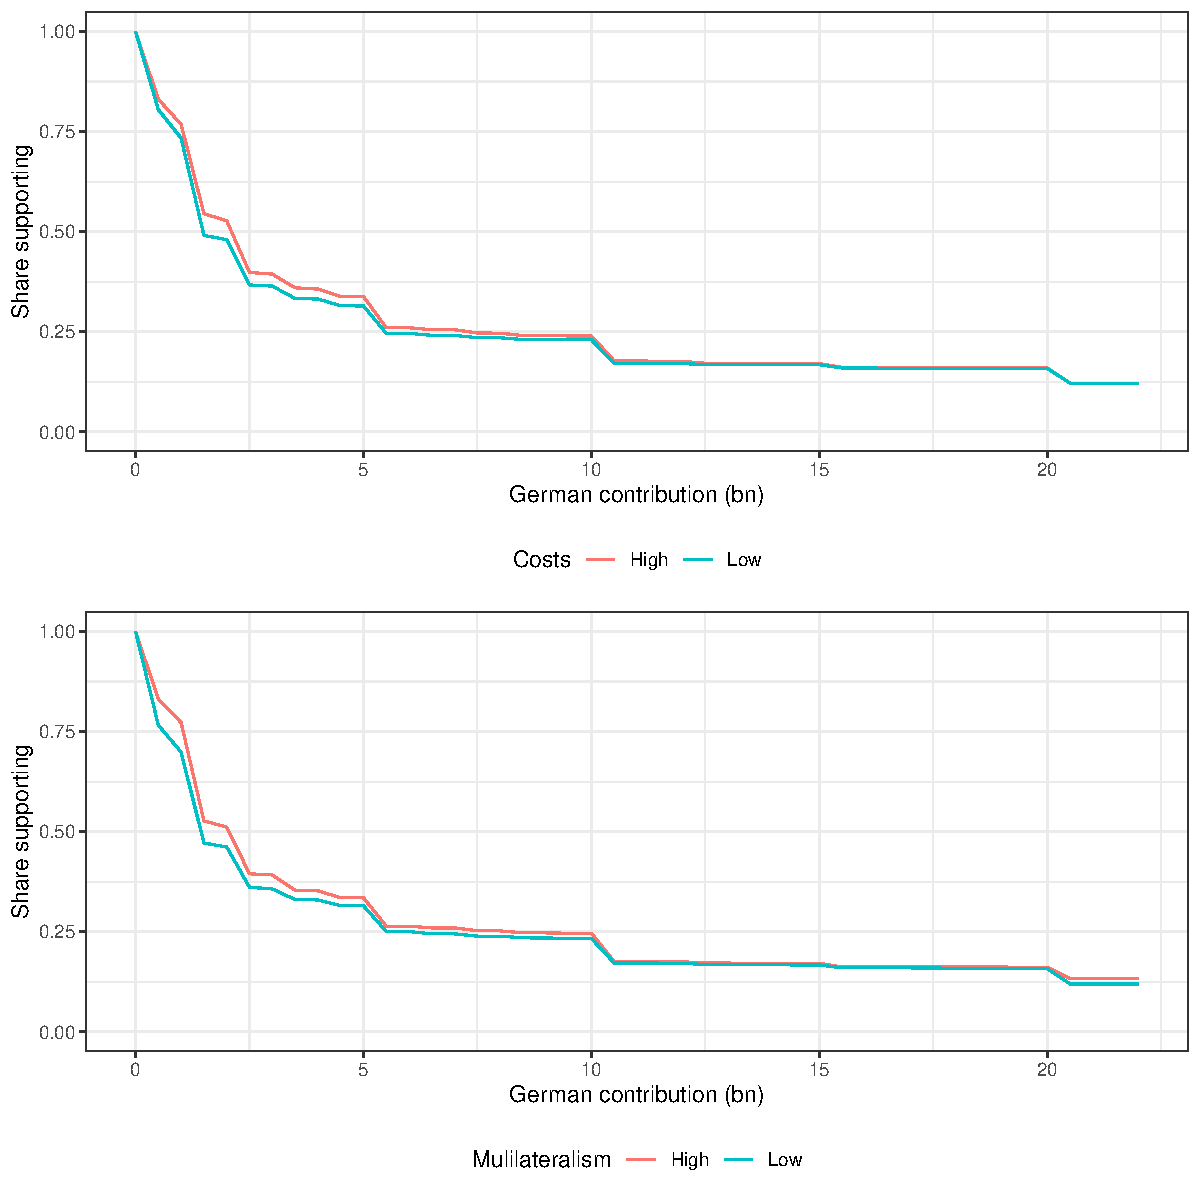
\includegraphics[width=\linewidth]{"../2_output/cumulative.pdf"}
	\caption{Distribution of support for contributions of different sizes}
	\label{fig:hist1}
	%\floatnote{This is a note for this figure.}
\end{figure}

Figure \ref{fig:main1} shows the marginal effects of all conditions on optimal cash donations and doses.

\begin{figure}[hbt!]
	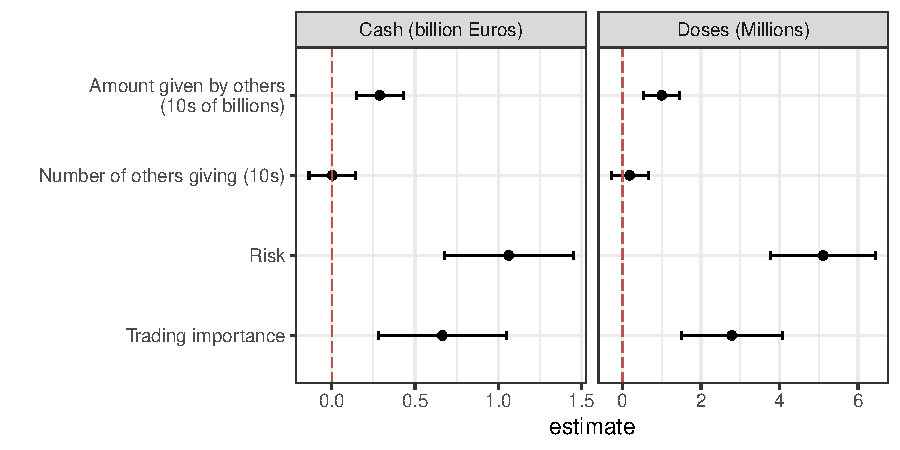
\includegraphics[width=\linewidth]{"../2_output/E1_main.pdf"}
	\caption{Results of Experiment 1}
	\label{fig:main1}
	%\floatnote{This is a note for this figure.}
\end{figure}

\textbf{Experiment 2}. 
Figure \ref{fig:conjoint_choice} reports the results of the treaty experiment. The results are largely in line with our theoretical expectations. 

The first result is somewhat inconsistent with findings so far: the number of vaccine doses that Germany would distribute to other countries negatively affects solidarity. Thus, citizens are more willing to share a smaller number of vaccine doses with other countries. In other words, international solidarity among citizens decreases with the absolute costs of distribution. 

Other results are largely in line with expectations. We find that it matters for citizens how much other countries are contributing to global vaccine redistribution. Solidarity among citizens is lowest when Germany contributes 20 per cent of all the vaccine doses that are globally shared, but it increases with other countries contributing a higher share to global vaccine sharing. In a similar fashion, we also find that the number of countries that participate in global vaccine sharing positively influences solidarity. Citizens are more willing to donate vaccine doses to poorer countries when more countries participate in global redistribution. With regard to the risk of infection, we show that citizens are more willing to share vaccine doses with poorer countries if these countries constitute a health risk for Germany (e.g. popular tourist destinations or countries with which Germany has strong economic ties). Thus, respondents were more willing to donate vaccine doses to minimize the risk of infections for Germany. 

While all these findings are in line with our theoretical expectations, the result for economic importance is counterintuitive. While we expected that the economic importance of a country for Germany should increase the willingness of citizens to share vaccine doses, we find the opposite effect here. The less important a country is to Germany economically, the more willing are citizens to redistribute vaccine doses. Hence, while all the other findings speak for a cost-benefit calculation that fundamentally drive international solidarity among citizens, this finding instead suggests that also the neediness of a country could account for the level of solidarity among citizens. 

\begin{figure}[hbt!]
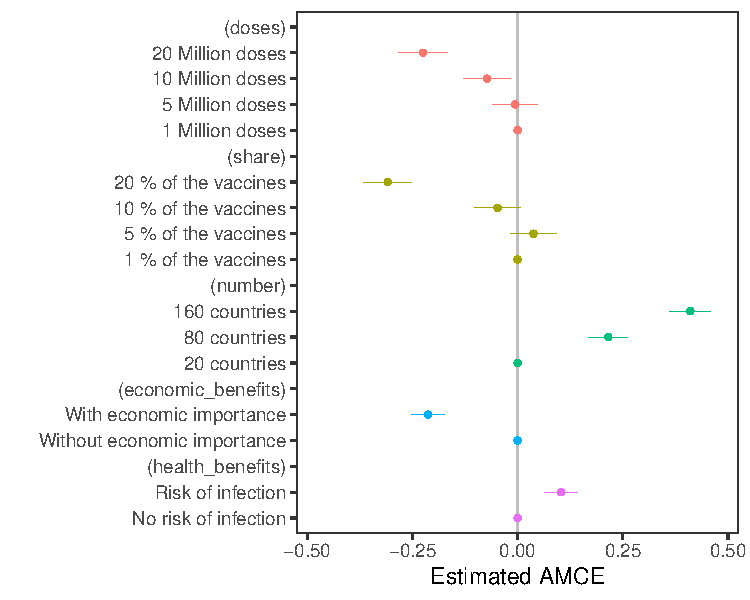
\includegraphics[width=\linewidth]{"../2_output/amces.pdf"}
\caption{Results of Experiment 2}
\label{fig:conjoint_choice}
%\floatnote{This is a note for this figure.}
\end{figure}

\begin{figure}[hbt!]
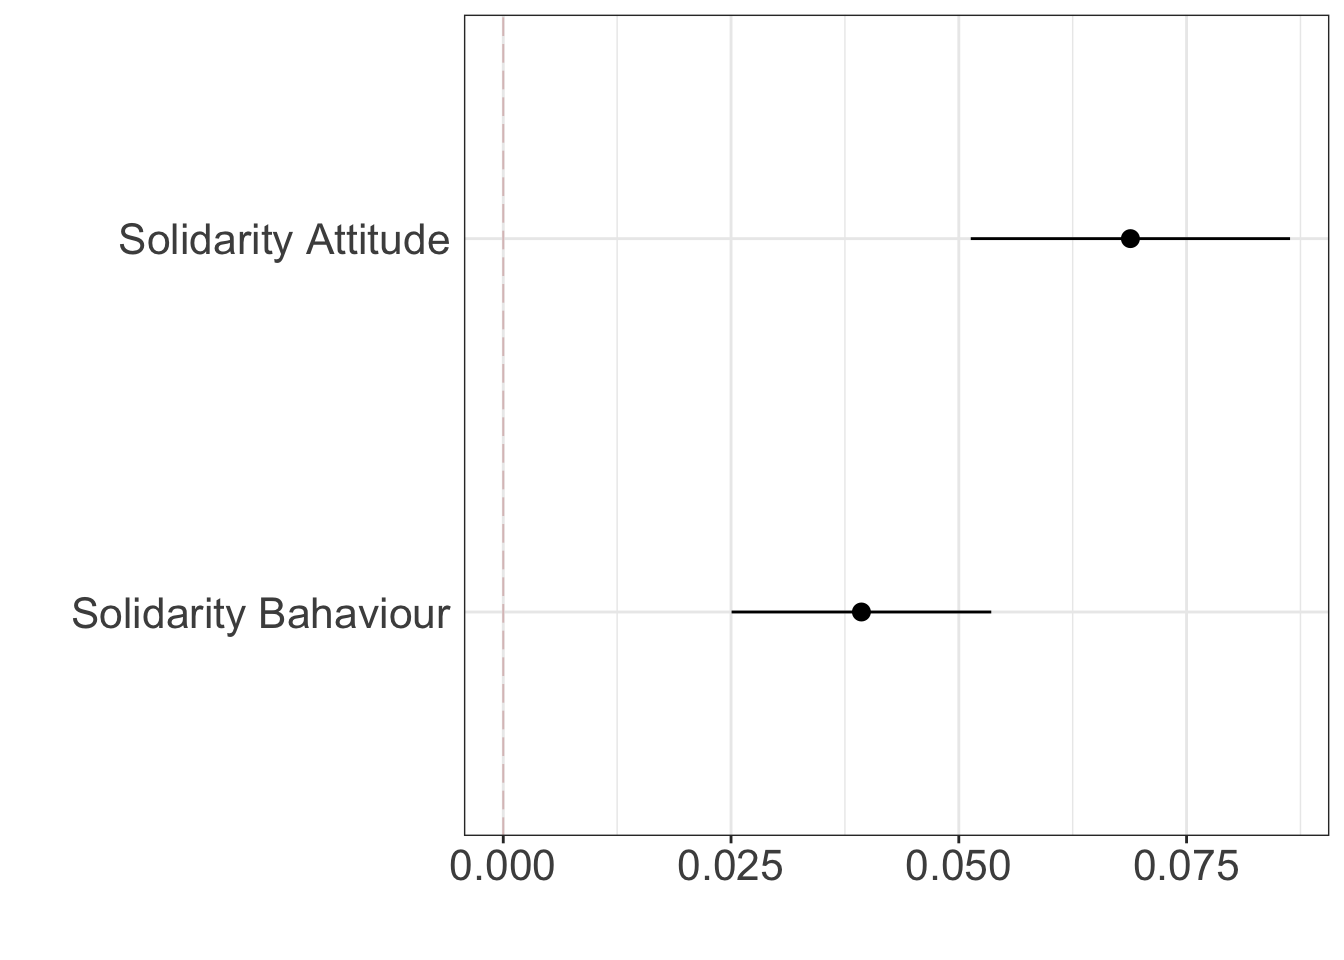
\includegraphics[width=\linewidth]{2_figures/fig_video.png}
\caption{Effect of video treatment on individual solidarity}
\label{fig:video}
%\floatnote{This is a note for this figure.}
\end{figure}


\textbf{Experiment 3}. Figure \ref{fig:video} reports the findings of the randomized intervention. We find that respondents in the treatment group which were exposed to the video are significantly more likely to show solidarity both with regard to the attitudinal and the behavioural outcome. More specifically, the willingness to personally support international distribution of vaccines is 0.069 units higher than in the control group. In a similar vein, the donations that respondents made to UNICEF were on average significantly higher in the treatment than in the control group. 

A final analysis examines how Experiment 3 alters the results on support for agreements assessed in Experiment 2. Table \ref{table:coefficients} gives the main results. We see clear evidence for the imact of the video on assessment of agreements. First we see that te video made respondents less likely to support ungenerous agreements (with low contributions, few donors, and small shares). Second the vide greatly mitigates, but does not overcome, the aversion to larger contributions. It greatly augments the desire to see more donors. Finally there is weak evidence that it weakens the strategic gains from health outcomes for Germany. 

These treatment effects do not persist to predict outcomes from Experiment 1


\begin{table}[h!]
\begin{center}
\begin{tabular}{l c c}
\hline
 & rating & choice \\
\hline
Constant (Average rating)                 & $0.172^{***}$  & $0.529^{***}$  \\
                                          & $(0.028)$      & $(0.007)$      \\
Video effect (given ungenerous agreement) & $-0.190^{***}$ & $-0.044^{***}$ \\
                                          & $(0.041)$      & $(0.010)$      \\
German contribution                       & $-0.101^{***}$ & $-0.030^{***}$ \\
                                          & $(0.009)$      & $(0.002)$      \\
German share                              & $-0.097^{***}$ & $-0.022^{***}$ \\
                                          & $(0.009)$      & $(0.002)$      \\
Number of donors                          & $0.165^{***}$  & $0.058^{***}$  \\
                                          & $(0.012)$      & $(0.003)$      \\
Economic benefits                         & $-0.209^{***}$ & $-0.053^{***}$ \\
                                          & $(0.020)$      & $(0.005)$      \\
Health benefits                           & $0.133^{***}$  & $0.036^{***}$  \\
                                          & $(0.020)$      & $(0.005)$      \\
Video * Contribution                      & $0.060^{***}$  & $0.020^{***}$  \\
                                          & $(0.013)$      & $(0.003)$      \\
Video * Share                             & $0.020$        & $0.002$        \\
                                          & $(0.013)$      & $(0.003)$      \\
Video * Donors                            & $0.095^{***}$  & $0.019^{***}$  \\
                                          & $(0.017)$      & $(0.004)$      \\
Video * Economics                         & $-0.011$       & $-0.008$       \\
                                          & $(0.028)$      & $(0.007)$      \\
Video * Health                            & $-0.048$       & $-0.014^{*}$   \\
                                          & $(0.028)$      & $(0.007)$      \\
\hline
R$^2$                                     & $0.015$        & $0.021$        \\
Adj. R$^2$                                & $0.015$        & $0.021$        \\
Num. obs.                                 & $82692$        & $82692$        \\
RMSE                                      & $2.033$        & $0.495$        \\
\hline
\multicolumn{3}{l}{\scriptsize{$^{***}p<0.001$; $^{**}p<0.01$; $^{*}p<0.05$}}
\end{tabular}
\caption{Effects of treatment on drivers of support for agreements. }
\label{table:coefficients}
\end{center}
\end{table}



\section{Conclusions and implications}


The numbers supported by the median German citizen, on the order of 2 billion Euros, if 



%%%%%%%%%%%%%

% HK: This paragraph could be shortened
%Next, we explore how CATE estimates behave when we change a single covariate, while keeping all the other covariates at some fixed value. In Fig. 3 we evaluate a variable of interest across quantiles, while keeping all other covariates at their median. T  We find a negative interaction effect between the high financial and increased freedoms treatment and the \textit{Age} of the respondents. While both treatment show significant effects for younger cohorts, they are less likely to yield significant effects for older subgroups. The possibility to get vaccinated at the local doctor yields slightly stronger predicted treatment effects for the older cohorts in the study. Using the causal forest, we also find evidence that attitudes towards the vaccination explain heterogeneity in the treatment effects. Those respondents who stated that they were \textit{undecided} to get vaccinated showed higher treatment effects for high financial incentives and personal freedoms. Further, increased personal freedoms are predicted to yield higher CATE's for those who show less \textit{solidarity} with others in the society (low values on the scale). The possibility to get vaccinated at the local doctor is more likely to yield treatment effects for those who show more solidarity with others. Lastly, we show that those who do not \textit{support social distancing} once they are vaccinated are also more likely to show strong treatment effects for increased personal freedoms. 






%% Use \bibliography{...} if using BibTeX
\bibliography{solidarity}
\bibliographystyle{apsr}

%TC:subst \printbibliography \bibliography
%TC:macro \field [0,1]
%TC:macro \name [0,0,0,1]
%TC:macro \list [0,0,1]
%% Use \printbibliography if using BibLaTeX
% \printbibliography

\clearpage
%%%%%%%%%%%%%%%%%%%%%%%%%%%%%%%%%%%%%%%%%%%%%%%%%%%%%%% 
\setcounter{page}{1}

\begin{center}
\appendix{\textbf{\Large{Supplementary Materials}}}
\end{center}


%\begin{center}
%\Large{What incentives can spur Covid-19 vaccination uptake?} \\
%\end{center}




%%%%%%%%%%%%%%%%%%%%%%%%%%%%%%%%%%%%%%%
\tableofcontents


\clearpage
\section{Study Design}


\begin{itemize}
\item
  \textbf{Introductory text}: And now we come to the topic of the global
  vaccination campaign. The pandemic can only be defeated if it is
  brought under control globally. In the fight against Covid-19, the
  provision of vaccines is particularly important. The COVAX platform
  was set up under the leadership of the World Health Organization (WHO)
  for the acquisition and fair distribution of vaccines.
\item
  \textbf{Video}: The video can be found here:
  https://www.dw.com/de/impfstoff-f\%C3\%BCr-entwicklungsl\%C3\%A4nder/av-56554104
\end{itemize}

\subsection{Outcome: Willingness to share}


\hypertarget{outcome-personal-donation}{%
\subsection{Outcome: Personal
donation}\label{outcome-personal-donation}}

\begin{itemize}
\item
  \textbf{Personal donation}: You can also contribute to the global
  distribution of the vaccines yourself. UNICEF is working on behalf of
  the COVAX initiative to ensure that the corona vaccines are made
  available to people in the poorest countries.

  Next to the 75 Mingle points that you receive for taking part in this
  survey, you will receive an \textbf{additional 50 Mingle points} from
  us. You can either keep these points yourself or donate all or part of
  them to UNICEF for the worldwide distribution of corona vaccines. For
  every mingle point you donate, we donate 1.5 mingle points to UNICEF.

  Please select how the additional Mingle points should be allocated to
  you or UNICEF.
\end{itemize}




\begin{longtable}[]{@{}lll@{}}
\caption{Bonuses and donations}
\label{table:mingle}
\endfirsthead
\endhead
\toprule
& Your Bonus & Donation to UNICEF\tabularnewline
\midrule
\endhead
1 & 0 Mingle Points & 75 Mingle Points\tabularnewline
2 & 10 Mingle Points & 60 Mingle Punkte\tabularnewline
3 & 20 Mingle Points & 45 Mingle Points\tabularnewline
4 & 30 Mingle Points & 30 Mingle Points\tabularnewline
5 & 40 Mingle Points & 15 Mingle Points\tabularnewline
6 & 50 Mingle Points & 0 Mingle Points\tabularnewline
\bottomrule
\end{longtable}


\begin{itemize}
\tightlist
\item
  \emph{Donations go here:}
  https://www.unicef.de/spenden/jetzt-spenden?purpose=235762
\end{itemize}

    \hypertarget{conjoint-design}{%
\subsection{Conjoint Design}\label{conjoint-design}}

\begin{itemize}
\tightlist
\item
  \textbf{Introductory text}: In the following, we present suggestions
  on how Germany's contribution to the global distribution of vaccine
  doses to poorer countries could look like this year.
\item
  \textbf{Conjoint Design}: Our second outcome measure is a conjoint experiment (two profiles) with randomly assigned factors (uniform) over five attributes. Each respondents will see three pairs. Unit of randomization is respondent pair.
\end{itemize}


subsection{Wave 2 conjoint results}

In wave 2 of the survey we implemented a Conjoint experiment in which respondents assessed two hypothetical proposals about Germany's contribution to global vaccine sharing. Respondents were asked  to indicate which proposal they would prefer and to rate each proposal with regard to how likely they would vote in favor of or against it in a referendum. The Conjoint experiment allows for estimating the effect of each factor on respondents' preferences for global vaccine sharing. We randomize the following dimensions: contribution to global vaccine sharing, contribution to global vaccine sharing relative to other countries, number of countries participating in global vaccine sharing, economic benefits and health benefits. The factors were assigned with independent probabilities. Each respondent received three vignettes successively. However, respondents did not see that same profile twice. 

This design differs from the wave 4 design in two important ways. First whereas in wave 4 outcomes included both contributions and doses; the wave 2 design focused on doses only and included the number of doses as part of the conjoint features. Second the economic and health risk items in the wave 2 conjoint implictly altered the *set* of countries receiving rather than the conditions under which countries receive. In addition the orders of magnitude are not in line with those facing policy makers. 



\begin{longtable}[]{@{}ll@{}}
\toprule
\begin{minipage}[b]{0.40\columnwidth}\raggedright
\strut
\end{minipage} & \begin{minipage}[b]{0.54\columnwidth}\raggedright
Proposal\strut
\end{minipage}\tabularnewline
\midrule
\endhead
\begin{minipage}[t]{0.40\columnwidth}\raggedright
Sharing of vaccination doses\strut
\end{minipage} & \begin{minipage}[t]{0.54\columnwidth}\raggedright
\{0\} Germany will give away 1 Million doses of its Covid Vaccine\strut
\end{minipage}\tabularnewline
\begin{minipage}[t]{0.40\columnwidth}\raggedright
\strut
\end{minipage} & \begin{minipage}[t]{0.54\columnwidth}\raggedright
\{1\} Germany will give away 5 Million doses of its Covid Vaccine\strut
\end{minipage}\tabularnewline
\begin{minipage}[t]{0.40\columnwidth}\raggedright
\strut
\end{minipage} & \begin{minipage}[t]{0.54\columnwidth}\raggedright
\{2\} Germany will give away 10 Million doses of its Covid Vaccine\strut
\end{minipage}\tabularnewline
\begin{minipage}[t]{0.40\columnwidth}\raggedright
\strut
\end{minipage} & \begin{minipage}[t]{0.54\columnwidth}\raggedright
\{3\} Germany will give away 20 Million doses of its Covid Vaccine\strut
\end{minipage}\tabularnewline
\begin{minipage}[t]{0.40\columnwidth}\raggedright
Germany's contribution compared to other countries\strut
\end{minipage} & \begin{minipage}[t]{0.54\columnwidth}\raggedright
\{0\} Germany contributes 1\% of the vaccines donated worldwide\strut
\end{minipage}\tabularnewline
\begin{minipage}[t]{0.40\columnwidth}\raggedright
\strut
\end{minipage} & \begin{minipage}[t]{0.54\columnwidth}\raggedright
\{1\} Germany contributes 5\% of the vaccines donated worldwide\strut
\end{minipage}\tabularnewline
\begin{minipage}[t]{0.40\columnwidth}\raggedright
\strut
\end{minipage} & \begin{minipage}[t]{0.54\columnwidth}\raggedright
\{2\} Germany contributes 10\% of the vaccines donated worldwide\strut
\end{minipage}\tabularnewline
\begin{minipage}[t]{0.40\columnwidth}\raggedright
\strut
\end{minipage} & \begin{minipage}[t]{0.54\columnwidth}\raggedright
\{3\} Germany contributes 20\% of the vaccines donated worldwide\strut
\end{minipage}\tabularnewline
\begin{minipage}[t]{0.40\columnwidth}\raggedright
How many countries share vaccination doses\strut
\end{minipage} & \begin{minipage}[t]{0.54\columnwidth}\raggedright
\{0\} 160 countries\strut
\end{minipage}\tabularnewline
\begin{minipage}[t]{0.40\columnwidth}\raggedright
\strut
\end{minipage} & \begin{minipage}[t]{0.54\columnwidth}\raggedright
\{1\} 80 countries\strut
\end{minipage}\tabularnewline
\begin{minipage}[t]{0.40\columnwidth}\raggedright
\strut
\end{minipage} & \begin{minipage}[t]{0.54\columnwidth}\raggedright
\{2\} 20 countries\strut
\end{minipage}\tabularnewline
\begin{minipage}[t]{0.40\columnwidth}\raggedright
Recipient countries - economic benefit\strut
\end{minipage} & \begin{minipage}[t]{0.54\columnwidth}\raggedright
\{0\} Countries in need with economic importance for Germany\strut
\end{minipage}\tabularnewline
\begin{minipage}[t]{0.40\columnwidth}\raggedright
\strut
\end{minipage} & \begin{minipage}[t]{0.54\columnwidth}\raggedright
\{1\} Countries in need, even without economic importance for
Germany\strut
\end{minipage}\tabularnewline
\begin{minipage}[t]{0.40\columnwidth}\raggedright
Recipient countries - risk of infection\strut
\end{minipage} & \begin{minipage}[t]{0.54\columnwidth}\raggedright
\{0\} Countries in need from which there is a risk of infection for
Germany\strut
\end{minipage}\tabularnewline
\begin{minipage}[t]{0.40\columnwidth}\raggedright
\strut
\end{minipage} & \begin{minipage}[t]{0.54\columnwidth}\raggedright
\{1\} Countries in need even if there is no risk of infection for
Germany\strut
\end{minipage}\tabularnewline
\bottomrule
\end{longtable}

\hypertarget{outcomes}{%
\subsection{Outcomes:}\label{outcomes}}

\begin{itemize}
\tightlist
\item
  \textbf{Forced Choice:} \emph{Displayed as bottom row in the conjoint
  table}

  \begin{itemize}
  \tightlist
  \item
    Which proposal do you prefer? (\emph{Respondents choose between both
    displayed options})
  \end{itemize}
\end{itemize}

\begin{itemize}
\tightlist
\item
  \textbf{Opposition to solidarity:} \emph{The following tables is
  displayed below the conjoint table}
\end{itemize}



\begin{figure}[hbt!]
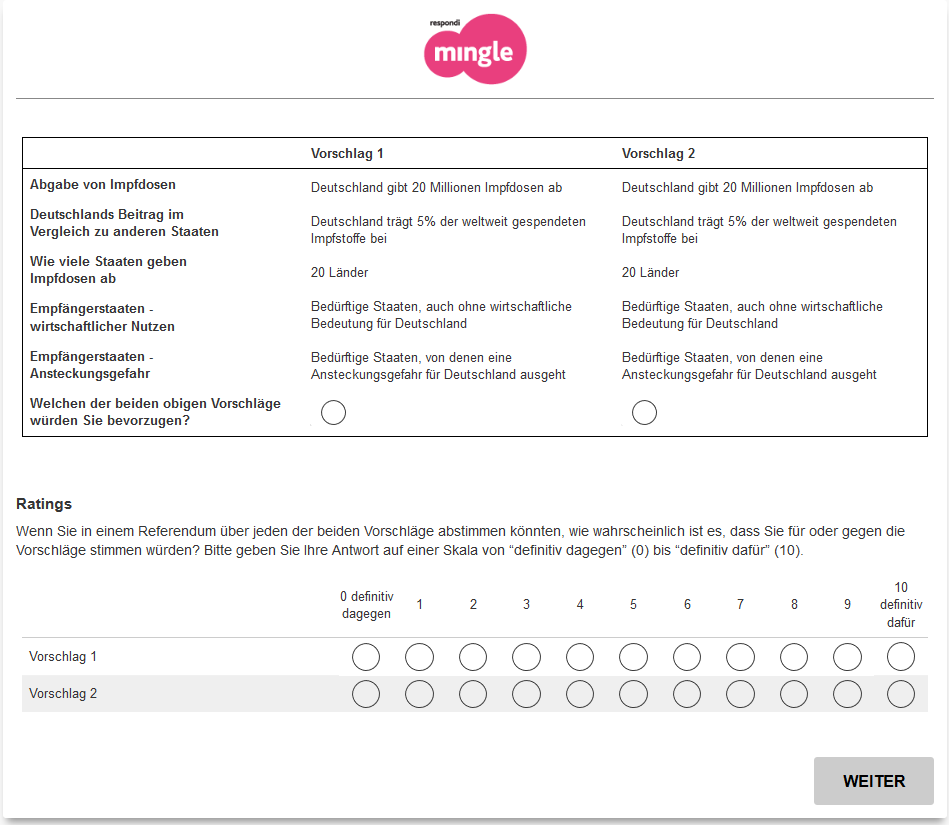
\includegraphics[width=\linewidth]{2_figures/screenshot.png}
\caption{Conjoint Design}
\label{fig:conjoint}

%\floatnote{This is a note for this figure.}
\end{figure}



\newpage
%%%%%%%%%%%%%%%%%%%%%%%%%%




\clearpage
\section{Descriptive Statistics}  

%%%%%%%%%%%%%%%%%




\end{document}